\chapter{Evaluatie}
\label{chap:evaluatie}

In dit hoofdstuk wordt de vergelijking uitgevoerd op basis van de vijf vergelijkingscriteria uit hoofdstuk \ref{chap:vergelijkingscriteria}, namelijk populariteit~(\ref{sec:evaluatie-populariteit}), productiviteit~(\ref{sec:evaluatie-productiviteit}), gebruik~(\ref{sec:evaluatie-gebruik}), ondersteuning~(\ref{sec:evaluatie-ondersteuning}) en performantie~(\ref{sec:evaluatie-performantie}). 
Daarna zullen deze vijf vergelijkingscriteria in sectie~\ref{sec:evaluatie-spinnenweb} worden samengevat.

%%%%%%%%%%%%%%%%%%%%%%%%%%%%%%%%%%%%%%%%%%%%%%%%%%%%%%%%%%%%%%%%%%%%%%%%

\section{Populariteit} % 2 blz inclusief google trends
\label{sec:evaluatie-populariteit}

De populariteit van de vier raamwerken op 8 mei 2013 wordt samengevat in tabel~\ref{tabel:evaluatie-populariteit}. 

\begin{table}[H]
\centering
\pgfplotstabletypeset[
  begin table=\begin{tabular}{p{8cm} p{1cm} p{1cm} p{1cm} p{1cm}},
  end table=\end{tabular},
  skip coltypes=true,
  col sep=comma,
  string type,
  header=true,
  columns={Populariteit,jQM,ST,Kendo,Lungo},
  columns/Populariteit/.style={column name=\textbf{Populariteit}, column type={l}},  
  columns/jQM/.style={column name=\textbf{\jqma}, column type={c}},
  columns/ST/.style={column name=\textbf{\sta}, column type={c}},
  columns/Lungo/.style={column name=\textbf{\lungoa}, column type={c}},
  columns/Kendo/.style={column name=\textbf{\kendoa}, column type={c}},
  every head row/.style={
    before row=\toprule,
    after row=\midrule},
  every last row/.style={
  	before row=\midrule,
    after row=\bottomrule}
]{tabellen/populariteit.csv}
\caption{Overzicht van populariteit op 8 mei 2013 voor \st{}~(\sta), \kendo{}~(\kendoa), \jqm{}~(\jqma) en \lungo{}~(\lungoa).}
\label{tabel:evaluatie-populariteit}
\end{table}

\kendo{} neemt de eerste plaats voor zich dankzij het zeer groot aantal vind-ik-leuks op \fb.
\jqm{} en \st{} slepen respectievelijk een tweede en derde plaats in de wacht, ondanks het feit dat ze in de literatuur de meest aangehaalde raamwerken zijn~\cite{David2011,Firtman2013,Hales2012,Oeflman2011}. 
Als laatste eindigt \lungo{} met een opmerkelijke lage populariteit op \so{} en \fb.
Bij het kijken naar de totaalscore kunnen twee groepen worden waargenomen, enerzijds de groep bestaande uit \kendo{} en \jqm{} en anderzijds de groep bestaande uit \st{} en \lungo{}.

Op Twitter heeft \jqm{} de meeste volgers, gevolgd door \kendo.
Op de voorlaatste plaats komt \lungo{}, maar als het aantal \term{tweets} wordt uitgezet ten opzichte van het aantal volgers, kan er gesteld worden dat \lungo{} het meest actief is.
\jqm{} en \kendo{} hebben een vergelijkbare activiteit bij het sturen van \term{tweets}.
\st{} heeft het minst aantal volgers en het aantal verstuurde \term{tweets} is slechts 1.

%TODO: als het open source is, zal het populairder zijn ??! verschil jQM/lungo <-> ST/Kendo door Github

In tegenstelling tot \jqm{} en \lungo{} bevinden \kendo{} en \st{} zich niet op \gh{}.
Zelfs indien \gh{} wordt weggelaten, blijft de rangschikking ongewijzigd.

\kendo{} verwijst op zijn website voor ondersteuning rechtstreeks naar de fora op \so{}. 
Toch blijft de populariteit van \kendo{} op \so{} lager dan die van \jqm{}.
\st{} behaalt de voorlaatste plaats, maar verbazender is \lungo{} die slechts een dertigtal vragen op \so{} heeft en dus op de laatste plaats eindigt.

\kendo{} en \jqm{} hebben beide een fanpgina op \fb{} opgericht in respectievelijk november 2011 en augustus 2010.
De fanpgina van \kendo{} heeft dus in een kortere tijd veel meer vind-ik-leuks opgeleverd dat de eerder opgerichte fanpgina van \jqm{}.
De verschillende producten van \kendo{} worden geaggregeerd op één fanpagina. 
\st{} en \lungo{} hebben enkel een interessepagina op \fb.
Dit verklaart het grote verschil in vind-ik-leuks op \fb.

Deze populariteit werd ook iedere week bijgehouden over een periode van een kleine twee maand en kan gevonden worden op figuur~\ref{fig:populariteit-evolutie}.
Opvallend is de sterke opmars van \kendo{} in deze korte periode.
Dit komt grotendeels door het enorm stijgend aantal \fb{} vind-ik-leuks.
De andere drie raamwerken stijgen gestaag.

%TODO vectorieel maken
\begin{figure}
  \centering
  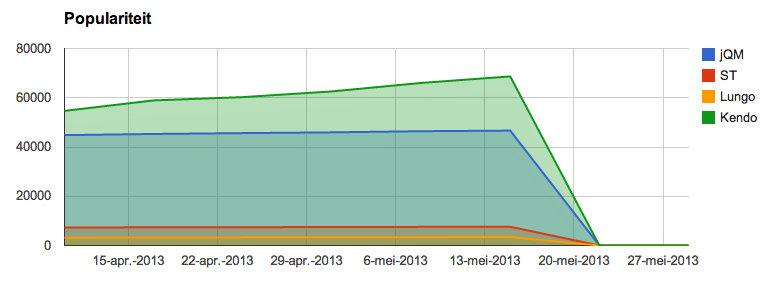
\includegraphics[width=\textwidth]{figuren/populariteit.png}
  \caption{Populariteit waargenomen over de periode van 15 april tot 22 mei 2013.}
  \label{fig:populariteit-evolutie}
\end{figure}

Als laatste wordt de populariteit aan de hand van Google Trends bekeken op figuur~\ref{fig:google-trends}.
Duidelijk is dat hier \jqm{} de grote winnaar is.
Sinds 2011 maakt het raamwerk een grote opmars door het uitbrengen van de eerste stabiele versie~1.0.
Eind 2012 kende \jqm{} echter een serieuze daling, maar deze werd terug een stijging omgezet door het uitbrengen van versie~1.3. 
\st{} kende een piek in maart 2012 bij het uitbrengen van \st{}~2.0.
Sinds begin 2012 maakt \kendo{} een opmars en als de trend zich verder zet, zal het \st{} inhalen.
Dit komt overeen met de waargenomen opmars van \kendo{} op figuur~\ref{fig:populariteit-evolutie}.
\lungo{} is nauwelijks op de grafiek waarneembaar.

%TODO voor Sander: kan jij die PDF met jouw matlab opnieuw genereren?
\begin{figure}[H]
  \centering
  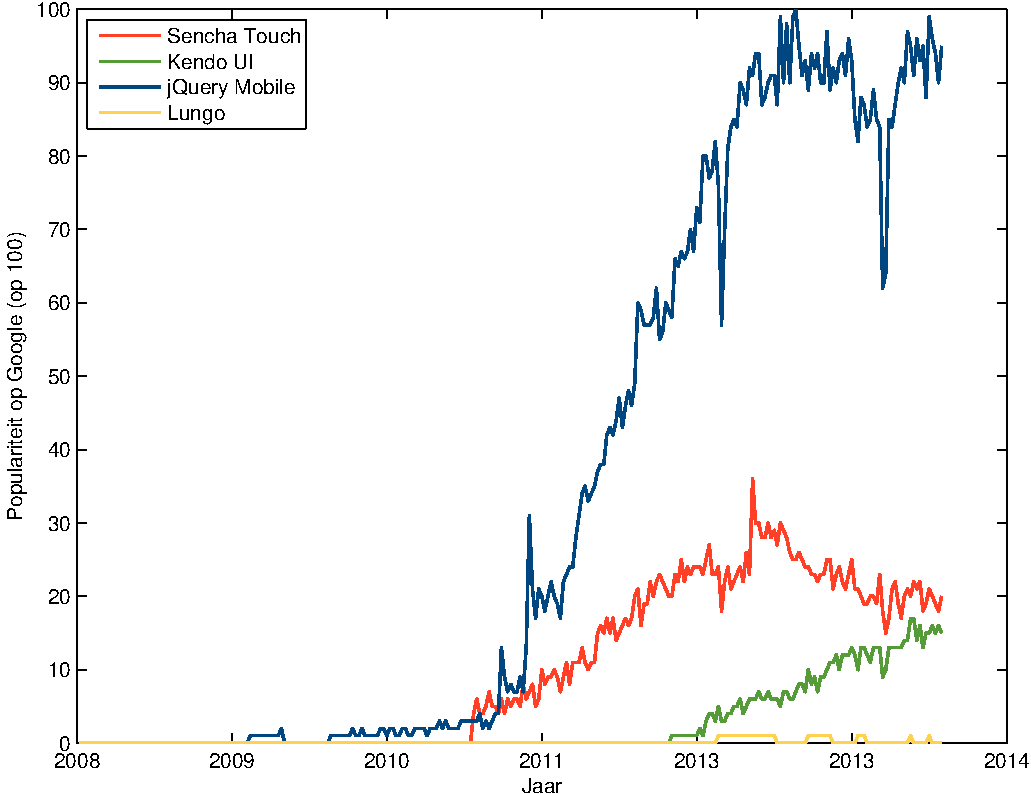
\includegraphics[width=\textwidth]{figuren/google-trends.pdf}
  \caption{Populariteit op Google Trends waargenomen van januari 2008 tot heden waarbij een resultaat van 100 overeenkomt met de grootste zoekinteresse~\cite{Google2012a}}
  \label{fig:google-trends}
\end{figure}